\section{讨论与结论}
\label{chapter:06}

% block-id: auto.06.p1
\hypertarget{auto.06.p1}{}
自动化研究的可复核性取决于任务与证据之间的连续关联。可见任务、工具事件、源码差异和确定性测试足以组织本文案例的执行记录；科学判断仍需要明确模型适用条件、比较量和验收容差。代码能够运行、图形能够生成和论文能够排版，分别对应软件执行、结果表达和文档构建，它们与物理可靠性通过验收步骤连接。

% block-id: auto.06.p2
\hypertarget{auto.06.p2}{}
研究过程同时涉及可编辑对象与稳定对象。参数、源码和后续研究任务需要便于修改；用于支撑结论的输入与结果则通过哈希固定。版本化数据目录保存原始文件身份，新运行写入独立目录。图件从保存数据重绘时记录来源与变换，双语稿件共享公式、图表和引用编号，使阅读层的变化可以追溯到同一科学内容。

% block-id: auto.06.p3
\hypertarget{auto.06.p3}{}
这种流程特别适合逐层推进的模型研究。解析和二维案例提供低成本回归，少股模型检查共同端约束，有限长度及三维路线逐步引入新的自由度。保存的几何与场数据为后续三维解释保留输入；真实中心线保留股线身份、弧长和局部位置，为后续模型扩展提供输入。结构性能比较还需匹配实际铜体积、回流、端区和数值不确定性。

% block-id: auto.06.figure
\hypertarget{auto.06.figure}{}
\begin{figure*}[!htbp]
\centering
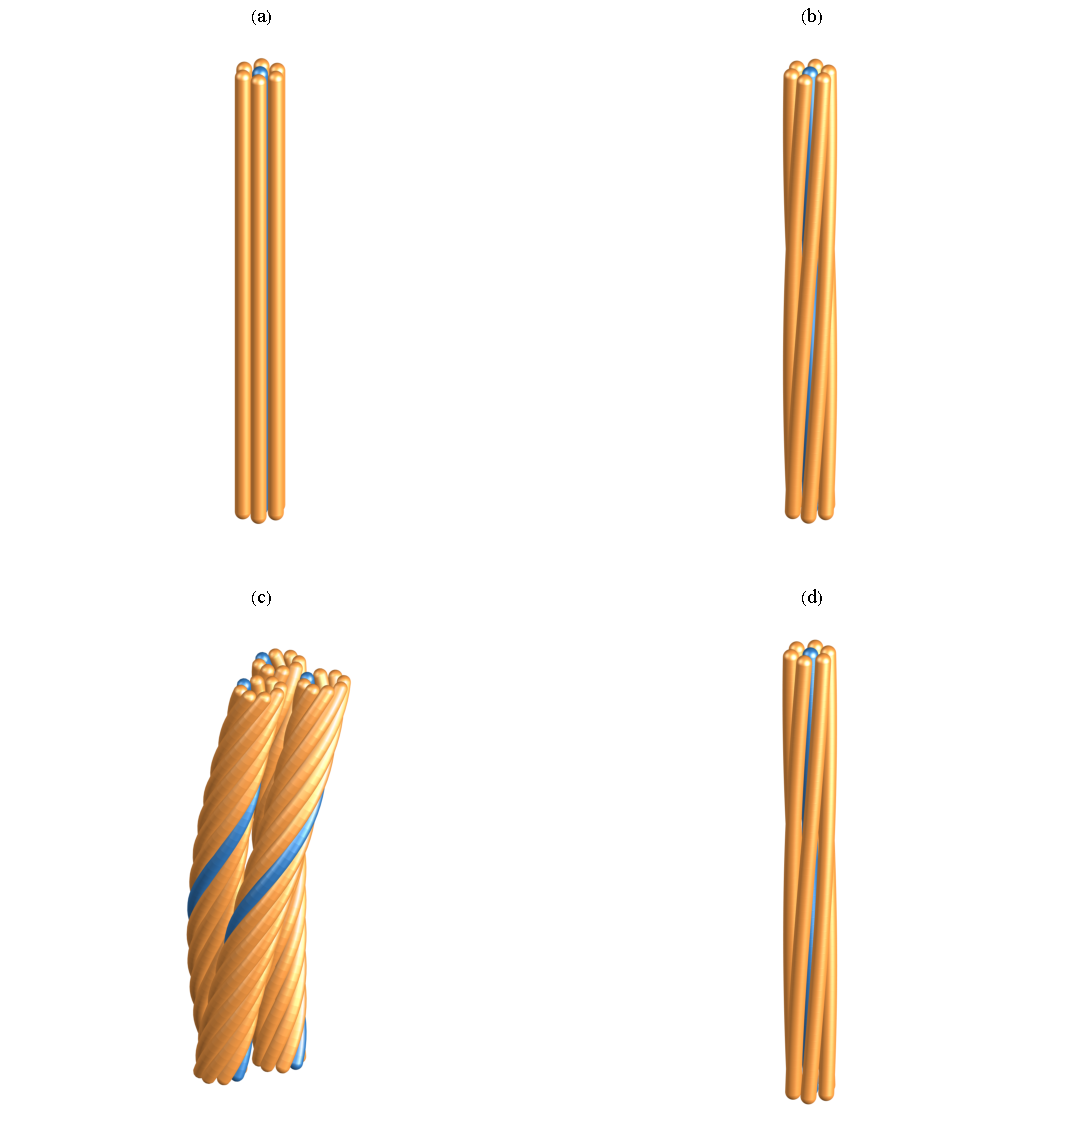
\includegraphics[width=\linewidth,height=.72\textheight,keepaspectratio]{../../assets/zh-CN/geometry_comparison.pdf}
\caption{股线中心线的三维结构比较。 面板依次展示直束、单级、传统多级局部和跨层结构。 24 股结构使用 0.100 mm 铜径，传统多级面板展示 3 mm 局部。蓝色标记保持选定股线的物理身份。}
\label{fig:geometry_comparison}
\end{figure*}

% block-id: auto.06.p4
\hypertarget{auto.06.p4}{}
本文交付了工作流、接入配置、运行适配、模型源码和可追溯案例。已有记录支持 Codex 通过 Wolfram 与 Ansys MCP 完成指定建模任务、扩展解析实现并依据错误证据修复接口；跨求解器和 A–φ 案例进一步说明验收状态如何限制结果解释。下一步方法评价可增加独立客户端、重复任务和人工基线，研究不同任务复杂度下的完成率、资源代价与修复稳定性。

% block-id: auto.06.p5
\hypertarget{auto.06.p5}{}
Wolfram、AgentTools、PyAEDT-MCP、PyAEDT 及相关开源数值与文档工具共同支持了本研究的实现。AI 参与源码检查、模型与适配代码、调用编排、诊断和文稿整理；作者负责物理假设、验收依据与研究结论。软件环境和上游来源随仓库提供，读者可沿方法、实现、测试和结果的索引继续研究。
